%% *****************************************************************************
%%
%% Alfresco PDF Sign - Installation Guide
%%
%% Description:
%% This document provides a comprehensive guide for the installation,
%% configuration, and verification of the Alfresco PDF Sign plugin.
%% The plugin enables PDF signing capabilities within Alfresco Community
%% Edition 7.4.2. Detailed instructions are provided to ensure successful
%% deployment and integration with your existing Alfresco environment.
%%
%% Author:
%% Rober de Avila Abraira
%%
%% Version:
%% 1.0.0
%%
%% Date:
%% 2024/08/20
%%
%% License:
%% This document is licensed under the Apache License, Version 2.0.
%% You may not use this file except in compliance with the License.
%% A copy of the License can be obtained at:
%% http://www.apache.org/licenses/LICENSE-2.0
%% Unless required by applicable law or agreed to in writing, this
%% document is distributed on an "AS IS" BASIS, WITHOUT WARRANTIES
%% OR CONDITIONS OF ANY KIND, either express or implied. See the
%% License for the specific language governing permissions and
%% limitations under the License.
%%
%% *****************************************************************************


\documentclass{template/ol-softwaremanual}

% Packages used
\usepackage[utf8]{inputenc} % for using Spanish characters
\usepackage{graphicx}  % for including images
\usepackage{microtype} % for typographical enhancements and better justification
\usepackage{ragged2e} % for justifying content
\usepackage{hyperref} % for hyperlinks
\usepackage{listings} % For code listings
\usepackage{xcolor} % For customizing colors
\usepackage[a4paper,top=4.2cm,bottom=4.2cm,left=3.5cm,right=3.5cm]{geometry} % for setting page size and margins

\renewcommand{\contentsname}{Contenido}

% Custom macros used in this example document
\newcommand{\doclink}[2]{\href{#1}{#2}\footnote{\url{#1}}}
\newcommand{\cs}[1]{\texttt{\textbackslash #1}}

% Frontmatter data; appears on title page
\title{Guía de Instalación \\ Alfresco PDF Sign}
\version{1.0.0}
\author{Rober de Avila Abraira}
\softwarelogo{
\includegraphics[width=8cm]{images/logo}}


\begin{document}

\maketitle

\tableofcontents
\newpage


\section{Introducción}

\textbf{Alfresco PDF Sign} es un plugin que ha sido desarrollado específicamente para añadir funcionalidades avanzadas de firma digital a documentos PDF dentro de la plataforma \textbf{Alfresco Community Edition 7.4.2}. Este plugin permite a los usuarios agregar firmas digitales visibles o invisibles a los documentos PDF almacenados en Alfresco, asegurando la autenticidad e integridad de los documentos.

Además, el plugin ofrece opciones para personalizar la ubicación de la firma, seleccionar diferentes certificados digitales, y automatizar el proceso de firma mediante reglas aplicadas a carpetas específicas. Estas capacidades son esenciales para garantizar la integridad y autenticidad de los documentos en flujos de trabajo que manejan información sensible o regulada.


\subsection{Objetivos de la guía}
Esta guía está diseñada para proporcionar instrucciones claras y detalladas para la instalación, configuración y verificación del plugin \textbf{Alfresco PDF Sign }en un entorno de \textbf{Alfresco Community Edition 7.4.2}. Al completar esta guía, serás capaz de:

\begin{itemize}
	\item Instalar y configurar el plugin \textbf{Alfresco PDF Sign} en tu entorno Alfresco.
	\item Verificar que la instalación se haya realizado correctamente y que el plugin esté funcionando como se espera.
\end{itemize}

\subsection{Audiencia destinada}
Esta guía está dirigida a administradores de sistemas o desarrolladores que trabaje con \textbf{Alfresco Community Edition 7.4.2} y necesite implementar la funcionalidad de firma digital en documentos PDF. Se asume que el lector tiene conocimientos básicos de administración de sistemas, manejo de servidores, y gestión de entornos Alfresco.

\subsection{Requisitos previos}
Para asegurar una instalación y configuración exitosa del plugin \textbf{Alfresco PDF Sign}, es esencial que el entorno cumpla con ciertos requisitos previos. A continuación, se detallan los requisitos del sistema:

\begin{itemize}
	\item \textbf{Alfresco Community Edition 7.4.2:} Asegúrate de que Alfresco, en la versión mencionada, esté instalado y funcionando correctamente antes de comenzar con la instalación del plugin.
	\item \textbf{Apache Tomcat 8.5+ (si se instala sin Docker):} Debe estar configurado como el contenedor de servlets para ejecutar Alfresco.
	\item \textbf{Maven (opcional):} Necesario si planeas compilar el plugin desde el código fuente.
	\item \textbf{Docker y Docker Compose (opcional)}: Útil si prefieres gestionar la instalación y el despliegue del plugin en contenedores, facilitando una configuración reproducible y fácil de gestionar.
\end{itemize}

\textbf{Nota:} Debes tener acceso administrativo al servidor donde está instalado Alfresco.

\section{Descarga del plugin}
Para instalar el plugin \textbf{ Alfresco PDF Sign}, primero debes obtener el archivo necesario. Existen dos opciones principales: descargar los archivos .amp precompilados o clonar el repositorio para compilar el plugin desde el código fuente. A continuación, se detallan ambos métodos.

\subsection{Descargar los archivos \textsl{.amp} precompilados}
La forma más sencilla y rápida de instalar el plugin es utilizando los archivos .amp precompilados. Estos archivos está listo para ser desplegado en tu entorno Alfresco sin necesidad de compilación adicional.

\begin{enumerate}
	\item \textbf{Accede a la sección de releases en GitHub:} Visita la página de \href{https://github.com/abraira85/alfresco-pdf-sign/releases}{releases} del proyecto en GitHub.
	\item \textbf{Selecciona la versión del plugin:} Busca la versión más reciente del plugin disponible en la lista de releases.
	\item \textbf{Descarga los archivos .amp:} Haz clic en el enlace de descarga para obtener los archivos .amp precompilados. Guarda estos archivos en una ubicación accesible en tu servidor donde está instalado Alfresco.
	\item \textbf{Preparación para la instalación:} Una vez descargado, puedes proceder con la instalación de los archivos .amp en Alfresco, utilizando ya sea Docker o Tomcat, según tus necesidades.
\end{enumerate}


\subsection{Clonar el repositorio para compilar desde el código fuente}
Si necesitas personalizar el plugin o prefieres construirlo desde el código fuente, puedes clonar el repositorio de GitHub y compilar los archivos .amp tú mismo.

\begin{enumerate}
	\item \textbf{Clonar el repositorio:} Abre una terminal en tu servidor y ejecuta el siguiente comando para clonar el repositorio:
\begin{lstlisting}[
	language=bash,
	frame=single,
	basicstyle=\ttfamily\scriptsize\color{white}, % Set text to white and slightly larger
	backgroundcolor=\color{black}, % Set background to black
	frame=single, % Frame around the code block
	framerule=0pt, % Remove the frame rule (optional)
	]
 git clone https://github.com/abraira85/alfresco-pdf-sign.git
\end{lstlisting}
	\item \textbf{Accede al directorio del proyecto:} Navega al directorio del proyecto clonado:
\begin{lstlisting}[
	language=bash,
	frame=single,
	basicstyle=\ttfamily\scriptsize\color{white}, % Set text to white and slightly larger
	backgroundcolor=\color{black}, % Set background to black
	frame=single, % Frame around the code block
	framerule=0pt, % Remove the frame rule (optional)
	]
 cd alfresco-pdf-sign
\end{lstlisting}
	\item \textbf{Compila y genera los ficheros \textsl{.amp}:} Si tienes Maven instalado, puedes compilar el plugin ejecutando: \\
{\small Compila el plugin para Alfresco.}
\begin{lstlisting}[
	language=bash,
	frame=single,
	basicstyle=\ttfamily\scriptsize\color{white}, % Set text to white and slightly larger
	backgroundcolor=\color{black}, % Set background to black
	frame=single, % Frame around the code block
	framerule=0pt, % Remove the frame rule (optional)
	]
 cd src/pdf-sign-repo/
 mvn clean install
\end{lstlisting}
\begin{lstlisting}[
	language=bash,
	frame=single,
	basicstyle=\ttfamily\scriptsize\color{white}, % Set text to white and slightly larger
	backgroundcolor=\color{black}, % Set background to black
	frame=single, % Frame around the code block
	framerule=0pt, % Remove the frame rule (optional)
	]
 [INFO] ------------------------------------------------------------------------
 [INFO] BUILD SUCCESS
 [INFO] ------------------------------------------------------------------------
 [INFO] Total time:  5.562 s
 [INFO] Finished at: 2024-08-21T07:20:54+02:00
 [INFO] ------------------------------------------------------------------------
\end{lstlisting}
{\small Retorna a la raíz del proyecto.}
\begin{lstlisting}[
	language=bash,
	frame=single,
	basicstyle=\ttfamily\scriptsize\color{white}, % Set text to white and slightly larger
	backgroundcolor=\color{black}, % Set background to black
	frame=single, % Frame around the code block
	framerule=0pt, % Remove the frame rule (optional)
	]
 cd -
\end{lstlisting}
{\small Compila el plugin para Alfresco Share.}
\begin{lstlisting}[
	language=bash,
	frame=single,
	basicstyle=\ttfamily\scriptsize\color{white}, % Set text to white and slightly larger
	backgroundcolor=\color{black}, % Set background to black
	frame=single, % Frame around the code block
	framerule=0pt, % Remove the frame rule (optional)
	]
 cd src/pdf-sign-share/
 mvn clean install
\end{lstlisting}
\begin{lstlisting}[
	language=bash,
	frame=single,
	basicstyle=\ttfamily\scriptsize\color{white}, % Set text to white and slightly larger
	backgroundcolor=\color{black}, % Set background to black
	frame=single, % Frame around the code block
	framerule=0pt, % Remove the frame rule (optional)
	]
 [INFO] ------------------------------------------------------------------------
 [INFO] BUILD SUCCESS
 [INFO] ------------------------------------------------------------------------
 [INFO] Total time:  2.372 s
 [INFO] Finished at: 2024-08-21T07:31:09+02:00
 [INFO] ------------------------------------------------------------------------
\end{lstlisting}
{\small Estos comandos generaran dos archivos .amp en el directorio target/amps de cada una de las carpetas. Copia estos archivos o otra carpeta para que lo uses luego en la instalación.}
\begin{lstlisting}[
	language=bash,
	frame=single,
	basicstyle=\ttfamily\scriptsize\color{white}, % Set text to white and slightly larger
	backgroundcolor=\color{black}, % Set background to black
	frame=single, % Frame around the code block
	framerule=0pt, % Remove the frame rule (optional)
	]
 src/pdf-sign-repo/target/pdf-sign-repo-1.0.0.amp
 src/pdf-sign-share/target/pdf-sign-share-1.0.0.amp
\end{lstlisting}
	\item \textbf{Preparación para la instalación:}	Una vez compilado, utiliza los archivos .amp generados para proceder con la instalación en tu entorno Alfresco, ya sea utilizando Docker o Tomcat.
\end{enumerate}


\section{Instalación directa en Tomcat}

\subsection{Preparación del entorno Tomcat}

\begin{enumerate}
	\item \textbf{Verificar el entorno de Alfresco:}
	\begin{itemize}
		\item Asegúrate de que Alfresco está instalado y funcionando correctamente en Tomcat.
		\item Detén el servicio de Alfresco para evitar problemas durante la instalación:
\begin{lstlisting}[
	language=bash,
	frame=single,
	basicstyle=\ttfamily\scriptsize\color{white}, % Set text to white and slightly larger
	backgroundcolor=\color{black}, % Set background to black
	frame=single, % Frame around the code block
	framerule=0pt, % Remove the frame rule (optional)
	]
 sudo service tomcat stop
\end{lstlisting}
	\end{itemize}
\end{enumerate}

\subsection{Instalación de los archivos \textit{.amp}}

\begin{enumerate}
	\item \textbf{Copiar los archivos \textit{.amp:}}
	\begin{itemize}
		\item Coloca los archivos \textit{.amp} en las siguientes ubicaciones dentro de la instalación de Tomcat:
		\begin{itemize}
			\item \textbf{pdf-sign-repo-1.0.0.amp:} Copia este archivo en el directorio amps/ para instalar el plugin en el repositorio Alfresco.
			\item \textbf{pdf-sign-share-1.0.0.amp:} Copia este archivo en el directorio amps\_share/ para instalar el plugin en la aplicación Alfresco Share.
		\end{itemize}
	\end{itemize}
	\item \textbf{Asegurar los permisos correctos:}
	\begin{itemize}
		\item Verifica que los archivos \textit{.amp} tengan los permisos adecuados para que Tomcat pueda acceder y aplicar los cambios.
	\end{itemize}
\end{enumerate}


\subsection{Aplicación de los archivos AMP}

\begin{enumerate}
	\item \textbf{Ejecutar el script \textit{apply\_amps.sh}:}
	\begin{itemize}
		\item Navega a la raíz de la instalación de Alfresco y ejecuta el siguiente comando para aplicar los archivos \textit{.amp}:
\begin{lstlisting}[
	language=bash,
	frame=single,
	basicstyle=\ttfamily\scriptsize\color{white}, % Set text to white and slightly larger
	backgroundcolor=\color{black}, % Set background to black
	frame=single, % Frame around the code block
	framerule=0pt, % Remove the frame rule (optional)
	]
 ./apply_amps.sh
\end{lstlisting}
		\item Este script instalará los módulos en Alfresco, integrando tanto el plugin en el repositorio como en la interfaz de usuario Share.
	\end{itemize}
\end{enumerate}

\subsection{Reinicio de Alfresco}

\begin{enumerate}
	\item \textbf{Reiniciar el servicio de Tomcat:}
	\begin{itemize}
		\item Reinicia el servicio Tomcat para que los cambios surtan efecto:
\begin{lstlisting}[
	language=bash,
	frame=single,
	basicstyle=\ttfamily\scriptsize\color{white}, % Set text to white and slightly larger
	backgroundcolor=\color{black}, % Set background to black
	frame=single, % Frame around the code block
	framerule=0pt, % Remove the frame rule (optional)
	]
 sudo service tomcat start
\end{lstlisting}
	\end{itemize}
	\item \textbf{Monitorear los Logs:}
	\begin{itemize}
		\item Revisa los logs de Tomcat para asegurarte de que la aplicación se inició sin errores:
\begin{lstlisting}[
	language=bash,
	frame=single,
	basicstyle=\ttfamily\scriptsize\color{white}, % Set text to white and slightly larger
	backgroundcolor=\color{black}, % Set background to black
	frame=single, % Frame around the code block
	framerule=0pt, % Remove the frame rule (optional)
	]
 tail -f /path/to/tomcat/logs/catalina.out
\end{lstlisting}
	\end{itemize}
\end{enumerate}


\subsection{Verificación de la instalación}

\begin{enumerate}
	\item \textbf{Acceder a Alfresco:}
	\begin{itemize}
		\item Una vez que Alfresco esté en funcionamiento, accede a través de \textit{http://<tu-servidor>:8080/alfresco}.
	\end{itemize}
	\item \textbf{Comprobar la funcionalidad del plugin:}
	\begin{itemize}
		\item Verifica que las funcionalidades proporcionadas por el plugin estén disponibles en \textbf{Alfresco Share}.
		\item Realiza una firma de prueba en un documento PDF para confirmar que el plugin está operando correctamente en ambas interfaces.
	\end{itemize}
\end{enumerate}


\section{Instalación en Alfresco montado sobre Docker}

Si ya tienes un entorno Alfresco ejecutándose en Docker, puedes seguir estos pasos para instalar los archivos AMP del plugin \textbf{Alfresco PDF Sign}.

\subsection {Parte 1: Instalación en el contenedor de Alfresco}

\begin{enumerate}
	\item \textbf{Verificar el entorno de Alfresco:}
	\begin{itemize}
		\item Asegúrate de que tu instancia de Alfresco está corriendo dentro de contenedores Docker. Usa el comando siguiente para verificar que los contenedores estén en funcionamiento:
\begin{lstlisting}[
	language=bash,
	frame=single,
	basicstyle=\ttfamily\scriptsize\color{white}, % Set text to white and slightly larger
	backgroundcolor=\color{black}, % Set background to black
	frame=single, % Frame around the code block
	framerule=0pt, % Remove the frame rule (optional)
	]
 docker ps
\end{lstlisting}
		\item Accede al contenedor de Alfresco:
\begin{lstlisting}[
	language=bash,
	frame=single,
	basicstyle=\ttfamily\scriptsize\color{white}, % Set text to white and slightly larger
	backgroundcolor=\color{black}, % Set background to black
	frame=single, % Frame around the code block
	framerule=0pt, % Remove the frame rule (optional)
	]
 docker exec -it <nombre_del_contenedor_alfresco> /bin/bash
\end{lstlisting}
	\end{itemize}
	\item \textbf{Copiar y aplicar el archivo AMP}
	\begin{itemize}
		\item Copia el archivo AMP correspondiente al repositorio (\textit{pdf-sign-repo-1.0.0.amp}) desde tu máquina local al contenedor:
\begin{lstlisting}[
	language=bash,
	frame=single,
	basicstyle=\ttfamily\scriptsize\color{white}, % Set text to white and slightly larger
	backgroundcolor=\color{black}, % Set background to black
	frame=single, % Frame around the code block
	framerule=0pt, % Remove the frame rule (optional)
	]
 # Sustituye el <nombre> por el nombre del contenedor de Alfresco.
 docker cp pdf-sign-repo-1.0.0.amp <nombre>:/usr/local/tomcat/amps/
\end{lstlisting}
		\item Aplica el archivo AMP en el repositorio utilizando la herramienta MMT:
\begin{lstlisting}[
	language=bash,
	frame=single,
	basicstyle=\ttfamily\scriptsize\color{white}, % Set text to white and slightly larger
	backgroundcolor=\color{black}, % Set background to black
	frame=single, % Frame around the code block
	framerule=0pt, % Remove the frame rule (optional)
	]
 java -jar /usr/local/tomcat/alfresco-mmt/alfresco-mmt*.jar install \
  /usr/local/tomcat/amps /usr/local/tomcat/webapps/alfresco \
  -directory -nobackup -force -verbose
\end{lstlisting}
	\end{itemize}
	\item \textbf{Ajustar los permisos y reiniciar el contenedor:	}
	\begin{itemize}
		\item Ajusta los permisos:
\begin{lstlisting}[
	language=bash,
	frame=single,
	basicstyle=\ttfamily\scriptsize\color{white}, % Set text to white and slightly larger
	backgroundcolor=\color{black}, % Set background to black
	frame=single, % Frame around the code block
	framerule=0pt, % Remove the frame rule (optional)
	]
 chgrp -R Alfresco /usr/local/tomcat/webapps \
   /usr/local/tomcat/amps /usr/local/tomcat/lib

 find /usr/local/tomcat/webapps -type d -exec chmod 0750 {} \;

 find /usr/local/tomcat/webapps -type f -exec chmod 0640 {} \;

 chmod -R g+r /usr/local/tomcat/webapps

 chmod 664 /usr/local/tomcat/amps/*
\end{lstlisting}
	\item Reinicia el contenedor:
\begin{lstlisting}[
	language=bash,
	frame=single,
	basicstyle=\ttfamily\scriptsize\color{white}, % Set text to white and slightly larger
	backgroundcolor=\color{black}, % Set background to black
	frame=single, % Frame around the code block
	framerule=0pt, % Remove the frame rule (optional)
	]
 docker restart <nombre_del_contenedor_alfresco>
\end{lstlisting}
	\end{itemize}
\end{enumerate}

\subsection {Parte 2: Instalación en el contenedor de Alfresco Share}

\begin{enumerate}
	\item \textbf{Acceder al contenedor de Alfresco Share:}
	\begin{itemize}
		\item Verifica que el contenedor de Alfresco Share esté corriendo:
\begin{lstlisting}[
	language=bash,
	frame=single,
	basicstyle=\ttfamily\scriptsize\color{white}, % Set text to white and slightly larger
	backgroundcolor=\color{black}, % Set background to black
	frame=single, % Frame around the code block
	framerule=0pt, % Remove the frame rule (optional)
	]
 docker ps
\end{lstlisting}
		\item Accede al contenedor de Alfresco Share:
\begin{lstlisting}[
	language=bash,
	frame=single,
	basicstyle=\ttfamily\scriptsize\color{white}, % Set text to white and slightly larger
	backgroundcolor=\color{black}, % Set background to black
	frame=single, % Frame around the code block
	framerule=0pt, % Remove the frame rule (optional)
	]
 docker exec -it <nombre_del_contenedor_share> /bin/bash
\end{lstlisting}
	\end{itemize}
	\item \textbf{Copiar y aplicar el archivo AMP de Share:}
	\begin{itemize}
		\item Copia el archivo AMP correspondiente a Share (\textit{pdf-sign-share-1.0.0.amp}) desde tu máquina local al contenedor:
\begin{lstlisting}[
	language=bash,
	frame=single,
	basicstyle=\ttfamily\scriptsize\color{white}, % Set text to white and slightly larger
	backgroundcolor=\color{black}, % Set background to black
	frame=single, % Frame around the code block
	framerule=0pt, % Remove the frame rule (optional)
	]
 # Sustituye el <nombre> por el nombre del contenedor de Alfresco Share.
 docker cp pdf-sign-share-1.0.0.amp <nombre>:/usr/local/tomcat/amps_share/
\end{lstlisting}
		\item Aplica el archivo AMP en Share utilizando la herramienta MMT:
\begin{lstlisting}[
	language=bash,
	frame=single,
	basicstyle=\ttfamily\scriptsize\color{white}, % Set text to white and slightly larger
	backgroundcolor=\color{black}, % Set background to black
	frame=single, % Frame around the code block
	framerule=0pt, % Remove the frame rule (optional)
	]
 java -jar /usr/local/tomcat/alfresco-mmt/alfresco-mmt*.jar install \
  /usr/local/tomcat/amps_share /usr/local/tomcat/webapps/share \
  -directory -nobackup -force -verbose
\end{lstlisting}
	\end{itemize}
	\item \textbf{Ajustar los permisos y reiniciar el contenedor:	}
	\begin{itemize}
		\item Ajusta los permisos:
\begin{lstlisting}[
	language=bash,
	frame=single,
	basicstyle=\ttfamily\scriptsize\color{white}, % Set text to white and slightly larger
	backgroundcolor=\color{black}, % Set background to black
	frame=single, % Frame around the code block
	framerule=0pt, % Remove the frame rule (optional)
	]
 chgrp -R Alfresco /usr/local/tomcat/webapps \
   /usr/local/tomcat/amps /usr/local/tomcat/lib

 find /usr/local/tomcat/webapps -type d -exec chmod 0750 {} \;

 find /usr/local/tomcat/webapps -type f -exec chmod 0640 {} \;

 chmod -R g+r /usr/local/tomcat/webapps

 chmod 664 /usr/local/tomcat/amps/*
\end{lstlisting}
	\item Reinicia el contenedor:
\begin{lstlisting}[
	language=bash,
	frame=single,
	basicstyle=\ttfamily\scriptsize\color{white}, % Set text to white and slightly larger
	backgroundcolor=\color{black}, % Set background to black
	frame=single, % Frame around the code block
	framerule=0pt, % Remove the frame rule (optional)
	]
 docker restart <nombre_del_contenedor_alfresco>
\end{lstlisting}
	\end{itemize}
\end{enumerate}


\section{Verificación de la instalación}

Después de instalar el plugin \textbf{Alfresco PDF Sign} en tu entorno Alfresco montado sobre Docker, es crucial verificar que la instalación se haya completado correctamente y que el plugin esté funcionando como se espera. Aquí, te explico cómo realizar una verificación sencilla utilizando la interfaz de \textbf{Alfresco Share}.

\begin{enumerate}
	\item \textbf{Acceder a Alfresco Share:}
	\begin{itemize}
	 	\item Abre un navegador web y ve a la URL: \\ \textit{http://<tu-servidor>:8080/share}
	 	\item Inicia sesión con tus credenciales de administrador.
	\end{itemize}
	\item \textbf{Comprobar los módulos desplegados:}
	\begin{itemize}
		\item Navega a la URL: \\ \textit{http://<tu-servidor>:8080/share/page/modules/deploy}
		\begin{figure}[h]
			\centering
			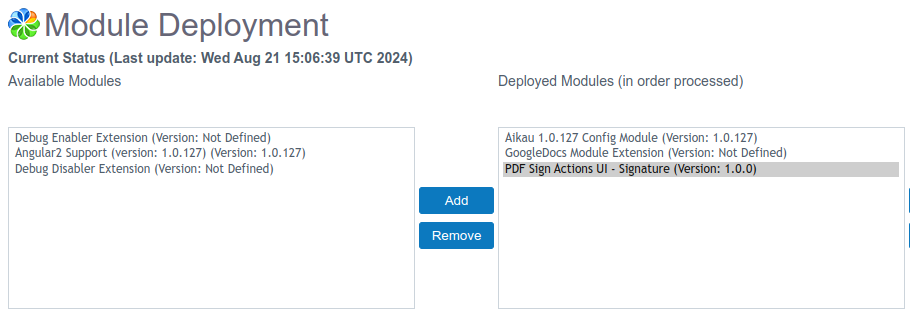
\includegraphics[width=\textwidth]{images/module}
			\label{fig:etiqueta_imagen}
		\end{figure}
		\item Verifica que el plugin Alfresco PDF Sign esté listado y activo.
	\end{itemize}
\end{enumerate}

\section{Recursos adicionales}

Para aprovechar al máximo el plugin \textbf{Alfresco PDF Sign}, es esencial acceder a recursos adicionales que ofrecen soporte técnico, documentación y herramientas útiles. A continuación, se incluyen enlaces clave y opciones de soporte para ayudarte a resolver dudas, solucionar problemas, y optimizar el uso del plugin y la plataforma Alfresco.

\subsection{Documentación relacionada}

\begin{itemize}
	\item \textbf{Guía de usuario de Alfresco}\\
	Documentación oficial de Alfresco, incluyendo guías para usuarios, administradores y desarrolladores.\\
	\url{https://docs.alfresco.com/}

	\item \textbf{Documentación del plugin Alfresco PDF Sign}\\
	Información detallada sobre la instalación, configuración y uso del plugin en su repositorio de GitHub.\\
	\url{https://github.com/abraira85/alfresco-pdf-sign/tree/master/docs}
\end{itemize}

\subsection{Enlaces útiles}

\begin{itemize}
	\item \textbf{Repositorio GitHub del plugin Alfresco PDF Sign}\\
	Acceso al código fuente, releases y más información sobre el plugin.\\
	\url{https://github.com/abraira85/alfresco-pdf-sign}

	\item \textbf{Comunidad Alfresco}\\
	Foro y comunidad de usuarios y desarrolladores de Alfresco para compartir conocimientos y resolver dudas.\\
	\url{https://hub.alfresco.com/}

	\item \textbf{Docker Hub - Alfresco Images}\\
	Página oficial de Alfresco en Docker Hub, con las imágenes Docker oficiales para Alfresco.\\
	\url{https://hub.docker.com/u/alfresco}
\end{itemize}

\section{Contacto}

Si tienes alguna pregunta, necesitas asistencia técnica, o deseas compartir tus comentarios sobre el plugin \textbf{Alfresco PDF Sign}, no dudes en ponerte en contacto con nosotros. Estamos aquí para ayudarte a sacar el máximo provecho de esta herramienta.

\begin{itemize}
	\item \textbf{GitHub}: Para reportar problemas, solicitar nuevas funcionalidades o contribuir al desarrollo del plugin, visita nuestro repositorio en GitHub: \url{https://github.com/abraira85/alfresco-pdf-sign}
\end{itemize}

Tu feedback y participación son esenciales para mejorar continuamente el plugin y asegurarnos de que cumpla con tus necesidades.


\end{document}
